\documentclass[pdflatex,sn-mathphys-num,iicol]{sn-jnl}

\usepackage{graphicx}
\usepackage{multirow}
\usepackage{amsmath,amssymb,amsfonts}
\usepackage{amsthm}
\usepackage[title]{appendix}
\usepackage{xcolor}
\usepackage{booktabs}
\usepackage{array}
\usepackage{float}
\floatstyle{ruled}
\newfloat{algorithm}{t}{loa}
\floatname{algorithm}{Algorithm}
% The algorithm/algpseudocode packages are not present in every TeX
% distribution, so the pseudocode below is typeset with built-in list
% machinery instead. This keeps the source compilable anywhere.

\newcolumntype{P}[1]{>{\raggedright\arraybackslash}p{#1}}

\theoremstyle{thmstyleone}
\newtheorem{theorem}{Theorem}
\newtheorem{proposition}[theorem]{Proposition}
\theoremstyle{thmstyletwo}
\newtheorem{example}{Example}
\newtheorem{remark}{Remark}
\theoremstyle{thmstylethree}
\newtheorem{definition}{Definition}

\raggedbottom

\begin{document}

\title[Equal Budgets, Unequal Airtime]{Equal Budgets, Unequal Airtime: Re-Evaluating
Event Triggers for Intermittently Connected Mobile Sensing}

\author*[1]{\fnm{Fatima Tu} \sur{Zahra}}\email{i232616@nu.edu.pk}

\author[1]{\fnm{Aleena} \sur{Zahra}}\email{i232514@nu.edu.pk}
\equalcont{These authors contributed equally to this work.}

\affil*[1]{\orgdiv{Department of Computer Science},
\orgname{National University of Computer and Emerging Sciences (FAST-NUCES)},
\orgaddress{\city{Islamabad}, \country{Pakistan}}}

\abstract{A mobile sensor surveying a pollutant plume over an intermittent link must decide
which readings are urgent enough to transmit and where to move in order to deliver them.
Content-aware triggers are usually evaluated against a value threshold under a matched
alarm budget, so that neither method gains simply by transmitting more. We show that this
matching can fail without any visible sign. Across 76{,}000 simulated missions and 332
paired comparisons, the hazard-threshold baseline cannot exceed about ten alarms per mission
at any setting, whereas a Gaussian-process urgency trigger reaches 148 in the same
configuration. Above this ceiling the budgets are equal in name only, and the urgency
trigger's advantage tracks how many more alarms it sends ($r=+0.861$). Where both triggers
send the same number of alarms, from 5 to 45 per mission, the threshold performs better in
77 of 79 cases (mean $-0.0516$ on-time ratio, 95\% CI $[-0.0572,-0.0459]$), a result that
replicates on held-out seeds and narrows from $-0.072$ to $-0.024$ as the budget grows. The
ceiling arises solely from tying the threshold's firing level to the hazard level; a
threshold allowed to fire below it sends 92 alarms per mission and ties the urgency trigger
at that budget. The method's clear benefit lies in routing: choosing where to upload from
improves the on-time ratio by 0.146. We recommend that matched-budget studies report the
alarm rates each method actually achieved.}

\keywords{event-triggered communication, mobile sensing, intermittent connectivity,
Gaussian process regression, unmanned aerial vehicles, experimental methodology}

\maketitle

%=====================================================================
\section{Introduction}\label{sec:intro}

An unmanned aerial vehicle (UAV) surveying a pollutant release cannot transmit everything
it measures. Radio coverage extends over only part of the area, the link fails in bursts,
and each reading has a deadline: it is valuable while a plume is moving towards a populated
zone and loses its value once the plume arrives. The agent must therefore decide
\emph{which} readings justify scarce airtime and \emph{where to move} to obtain a link good
enough to deliver them.

An obvious design ranks readings by how surprising and how hazardous they are and spends
the communication budget on the highest-ranked ones. An obvious baseline is far simpler:
transmit whenever the measured concentration exceeds a hazard level, the send-on-delta idea behind
event-triggered sampling~\cite{miskowiczSendOnDelta2006,
hakandurakEfficientEventBasedSampling2026}. Because a rule that fires more often will
deliver more, the two are normally compared under a \emph{matched alarm budget}: each
rule's trigger is tuned until both fire at the same rate, so any remaining difference
comes from \emph{which} readings each one picks.

This paper shows that the matching does not always hold and that the usual procedure does
not reveal the failure. We have not audited other studies; the case we can document is our
own, in which it turned a genuine deficit into an apparent advantage of up to $+0.104$.
Four findings follow from 76{,}000 simulated missions.

\begin{enumerate}
\item \textbf{The threshold baseline has a hard alarm ceiling.} At a trigger of zero it
already sends on every hazard crossing it sees, and still sends only 8.50 alarms per
mission. The urgency trigger reaches 148 in the same setting.
\item \textbf{Above the ceiling, a matched budget is matched in name only.} A request for
45 alarms still yields about 10, so the comparison measures additional airtime.
Over 332 paired comparisons, the urgency trigger's margin follows how many more
messages it sends ($r = +0.861$), even at a fixed budget.
\item \textbf{When airtime is genuinely equal, the simple baseline performs better}, in 77 of 79 cases,
and the urgency trigger is also 7.2 ticks slower. This holds from 5 to 45 alarms per
mission, across nine experimental factors, and on seeds never used for tuning.
\item \textbf{The ceiling is a consequence of the baseline's parameterisation, not of
threshold triggering.} Allowing the threshold to fire below the hazard level removes it:
that variant sends 92 alarms when asked for 90 and ties the urgency trigger at that budget,
and the urgency trigger's large lead over the capped baseline (0.747 against 0.402) largely
disappears.
\end{enumerate}

\paragraph{Contributions} (i) A direct measurement of a threshold trigger's alarm ceiling,
and a test showing the ceiling disappears when the firing level is set separately
(Sections~\ref{sec:saturation} and~\ref{sec:capacity}). (ii) Evidence over 332
comparisons that matched-budget evaluation stops being matched above that ceiling, so the
reported margin measures extra messages rather than better choices
(Section~\ref{sec:outspend}). (iii) A pre-registered test whose success rule was not met,
reported as not met, with the experiments that explain why (Sections~\ref{sec:prereg}
and~\ref{sec:equal}). (iv) Evidence that the routing component, choosing where to upload
from on a coverage map discovered in flight, is the method's clear benefit, worth 0.146
on-time ratio (Section~\ref{sec:ablation}).

%=====================================================================
\section{Related Work}\label{sec:related}

Four lines of work are relevant. Each optimises a quantity other than the timely delivery
of hazard readings.

\paragraph{Age of Information.} Age of Information (AoI)~\cite{kaulRealTimeStatus2012}
measures how old the newest delivered update is. AoI-optimal path planning for aerial
platforms~\cite{xieAoIoptimalPathPlanning2025, AoIOptimalMultiAAVEnabledISAC} and
distributed two-dimensional AoI~\cite{fidler2DAoIAgeofInformationDistributed2026} keep
this age low. For hazard monitoring the problem is that AoI ignores content: a stale
reading of clean air is penalised exactly as a stale reading of a hazardous plume. Two refinements
address this. Age of Incorrect Information~\cite{maatoukAgeIncorrectInformation2020}
counts age only while the receiver's picture is wrong, and Urgency of
Information~\cite{zhengUrgencyOfInformation2020} weights age by a context-dependent cost,
the closest relative of our urgency score (Eq.~\eqref{eq:urgency}). Ours differs in being
computed against an explicit model of what the receiver currently holds, and in driving
the agent's movement as well as its transmissions. We implement plain age-based sending as
the \texttt{time\_urg} baseline.

\paragraph{Informative path planning.} These methods choose paths that most reduce
uncertainty in a learned map~\cite{maAdaptiveInformativePath2025,
blanchardInformativePathPlanning2022}, often with Gaussian processes. Related work adapts
the sampling rate to platform movement~\cite{hanMobilityentropyawareAdaptiveUWB2026} or
uses learned sensing pipelines~\cite{calistiDeepLearningdrivenSensing2026}. Their goal is
map quality or sampling cost, not delivery, and Section~\ref{sec:ablation} shows that in
our setting a better map comes with worse timeliness.

\paragraph{Communication-aware trajectory planning.} Connectivity-aware UAV
routing~\cite{mardaniCommunicationAwareUAVPath2019, chuTrajectoryOptimizationResource2026,
hayatMultiobjectiveDronePath2020} optimises throughput or outage and usually assumes the
coverage map is known. Team-based methods plan for several UAVs under sparse
coverage~\cite{conceicaoPathPlanningOptimisation2026, liuTrajectoryPlanningTracking2026}.
The single agent considered here has no prior coverage map and must discover it in
flight.

\paragraph{Event-triggered sampling.} Sending only when a signal crosses a
threshold~\cite{hakandurakEfficientEventBasedSampling2026} is the direct source of our
baseline. This work reports how many transmissions are saved, but as far as we know not
that the rule has a \emph{ceiling} on how many it can produce, which is what we measure.

We adopt, rather than compete with, fast GP estimation~\cite{munozGaussianProcessesFast2023}:
fixed hyperparameters and a sliding window keep GP cost near 20\% of runtime.
Table~\ref{tab:related} summarises the comparison.

%=====================================================================
\section{Proposed Methodology}\label{sec:method}

\subsection{Problem formulation}

A single agent moves on an $n \times n$ grid for $T$ time steps (ticks). A pollutant field
$c(\mathbf{x}, t)$ spreads by advection and diffusion,
\begin{equation}
\frac{\partial c}{\partial t} = -\mathbf{u}\cdot\nabla c + D\nabla^2 c + s(\mathbf{x},t),
\label{eq:pde}
\end{equation}
with wind $\mathbf{u}$, diffusivity $D$ and a pulsing source $s$. At each tick the agent
observes the field, with noise, only at its current cell.

An \emph{event} is a cell whose true concentration crosses a hazard level $h$. Its
deadline is the time the plume takes to travel from that cell to a sensitive zone along
the wind; cells not upwind of the zone are never urgent. The events and deadlines depend
only on the field, never on the method, so every method answers the same question.

The agent maintains two Gaussian process (GP) models over $(x, y, t)$: its own, fitted to
everything it has measured, and a \emph{cloud-belief} GP fitted only to data it has
actually delivered. Urgency is evaluated against the cloud belief, so that it reflects what the
operator currently holds rather than what the agent itself knows.

The main measure is the \textbf{on-time ratio}: the fraction of observable events whose
hazard crossing reaches the cloud map before the deadline. The second is \textbf{mean
latency} in ticks.

\subsection{The urgency score}

For a reading $o$ at a cell where the cloud belief has mean $\mu$ and standard deviation
$\sigma$,
\begin{equation}
U = w_s\,\frac{|o - \mu|}{\max(\sigma, \sigma_{\min})}
  + w_c\,\frac{\max(0,\; o - h)}{\kappa}.
\label{eq:urgency}
\end{equation}
The first term is \emph{surprise}, scaled by the model's own uncertainty; the second is
\emph{consequence}, with scale $\kappa$. The terms are added rather than multiplied,
because a product vanishes wherever the model is uncertain and would then disregard a
reading far above the hazard level.

An alarm fires when $U$ stays above a trigger $\tau$ for $k=3$ ticks in a row. This
consistency gate applies to every content-based rule, so that no rule benefits merely from
lacking it. Urgency sets a deadline between 24 and 4 ticks through a percentile map; a linear map
put 62\% of deadlines at the limit because urgency values are heavy-tailed.

\subsection{Delivery and the decision rule}

The channel is a Gilbert--Elliott model: a two-state Markov chain that produces losses in
bursts. A short \emph{alert} needs one good tick, but the \emph{full upload} that updates
the cloud needs three good ticks in a row, or one with link quality $\geq 0.80$. Only full
uploads count as delivery.

At each tick the agent compares transmitting in place, exploring, and flying to any coverage
region it has found. For each option it simulates 200 link traces along the path to
estimate the probability of completing an upload before the deadline and the expected time. It
has no initial coverage map: cells where measured link quality exceeds 0.5 are marked
covered and grouped into regions. Figure~\ref{fig:arch} shows the architecture and
Algorithm~\ref{alg:loop} the per-tick loop.

\begin{figure*}[t]
\centering
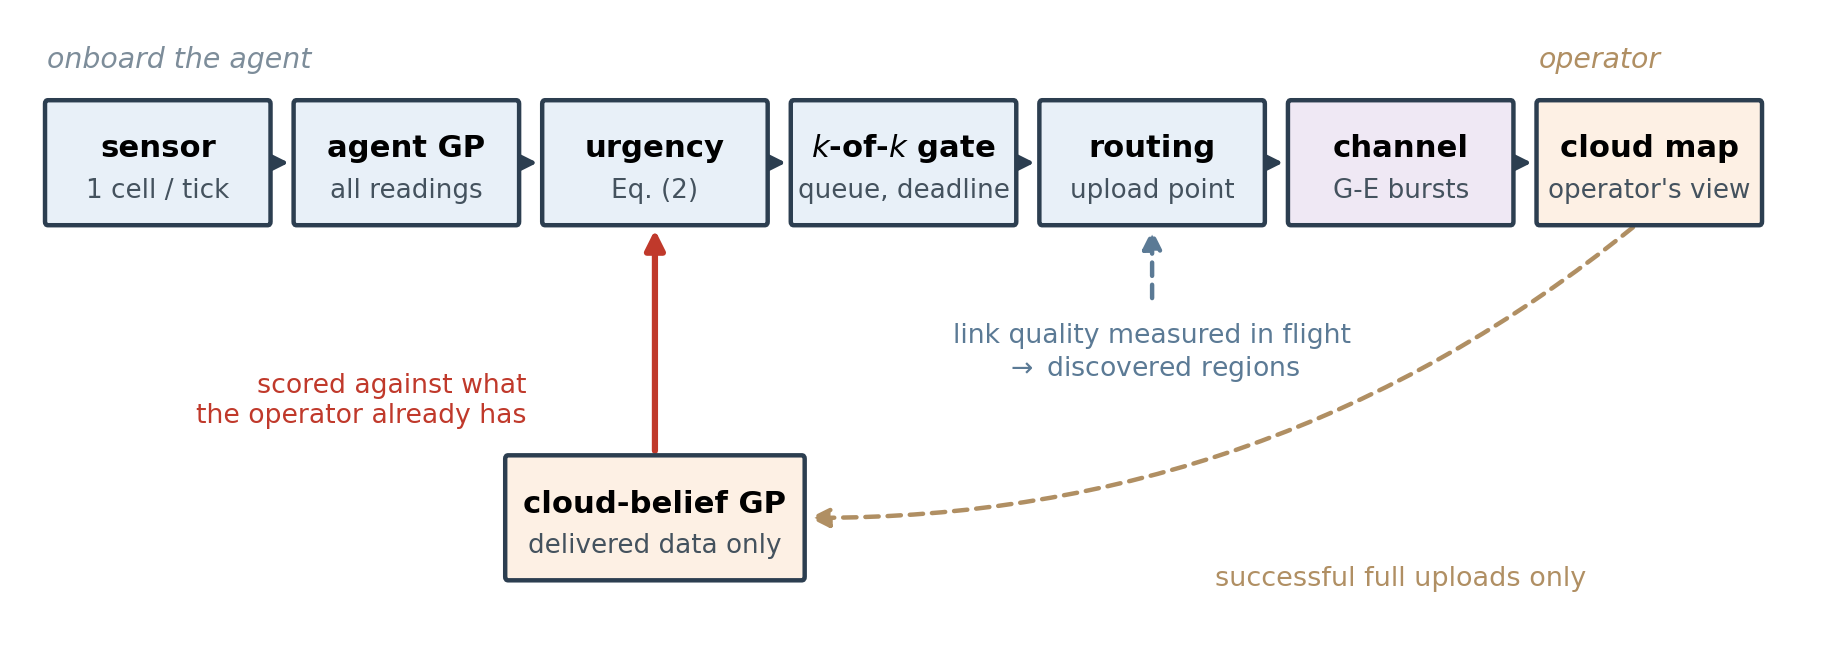
\includegraphics[width=\textwidth]{figs/fig_architecture.png}
\caption{System architecture. The agent maintains two GPs: its own, fitted to everything it
measures, and a cloud-belief GP fitted only to delivered data. Urgency is scored against
the cloud belief (red), that is, against what the operator already has. Only full uploads
update it.}\label{fig:arch}
\end{figure*}

\begin{algorithm}[t]
\caption{One mission tick. Lines 3--5 are the trigger; lines 7--9 are the routing.}\label{alg:loop}
\footnotesize
\begin{tabular}{@{}r@{\hspace{0.6em}}P{0.88\columnwidth}@{}}
1 & observe $o$ at the current cell; add it to the agent's own GP \\
2 & $(\mu, \sigma) \leftarrow$ cloud-belief GP at this cell \\
3 & $U \leftarrow$ Eq.~\eqref{eq:urgency} \\
4 & \textbf{if} $U > \tau$ on $k$ consecutive ticks \textbf{then} \\
5 & \quad queue the reading with a deadline derived from $U$ \\
6 & update the coverage regions from measured link quality \\
7 & \textbf{for each} option: transmit here, explore, move to region $r$ \\
8 & \quad simulate 200 link traces $\rightarrow$ $P(\text{on time})$, $E[\text{time}]$ \\
9 & execute the best option; attempt transmission \\
10 & \textbf{if} a full upload completes \textbf{then} update the cloud-belief GP \\
\end{tabular}
\end{algorithm}

%=====================================================================
\section{Experimental Setup}\label{sec:setup}

\subsection{Data}

The data are simulated. Equation~\eqref{eq:pde} is solved on a $40\times40$ grid for 800
ticks with an upwind scheme, using the combined stability limit
$\Delta t \leq 1/(|u|/\Delta x + |v|/\Delta x + 4D/\Delta x^2)$ and automatic
sub-stepping. The source pulses about every 110 ticks; a constant source settles into a
steady state and stops producing new hazard crossings.

Each seed is a different plume realisation: source position, wind speed and direction, and pulse
period all vary. There are two field scenarios, \emph{predictable} (steady wind) and
\emph{unpredictable} (an $80.2^\circ$ wind shift at tick 347 and a surprise second source
at tick 427), and two connectivity scenarios, \emph{sparse} (13.3\% of cells usable) and
\emph{dense} (33.4\%). A cell is usable when its per-attempt delivery probability,
including the channel's average factor of 0.768, exceeds 0.5.

\subsection{Calibration and the matched budget}

Before each comparison, every method's trigger is tuned by bisection until it fires at the
target rate. \textbf{The achieved rate is measured and reported, never assumed}, and
flagged if it is more than 10\% off target. Most experiments were tuned with 8 seeds;
re-tuning the key cells with 20 moved their mean margin from $-0.0605$ to $-0.0585$ and
changed no cell's sign.

\subsection{Seeds, statistics and reproducibility}

Calibration, evaluation and replication use separate seed blocks (5000--5299, 6000--6099
and 7000--7299), checked to have no overlap. Methods are compared on the same seeds with
the Wilcoxon signed-rank test, with 95\% confidence intervals and Holm correction within
each family. Every result row records the git commit, a configuration hash and library
versions, and the raw runs are committed, so every table and figure can be regenerated
without re-simulating. Runs used an Intel i7-1255U, Python 3.12.3, numpy 1.26.4, scipy
1.11.4 and scikit-learn 1.9.1; 93 regression tests cover the simulator.

\subsection{Methods compared}

Each method differs from the urgency trigger in exactly one component (Table~\ref{tab:methods}).

\begin{table}[t]
\caption{Methods compared. Bold marks the one part that differs from \texttt{proposed}.}
\label{tab:methods}
\centering
\footnotesize
\setlength{\tabcolsep}{3pt}
\begin{tabular}{@{}lll@{}}
\toprule
\textbf{Key} & \textbf{Trigger / change} & \textbf{Role} \\
\midrule
\texttt{proposed} & surprise $+$ consequence & urgency trigger \\
\texttt{threshold} & \textbf{value $>$ hazard} & B2, main baseline \\
\texttt{threshold\_dec} & \textbf{value $>\theta$, $\theta$ free} & B2d, decoupled \\
\texttt{time\_urg} & \textbf{time since delivery} & B3, AoI-style \\
\texttt{always\_tx} & \textbf{sends in place} & B1, no routing \\
\texttt{fixed\_dl} & \textbf{fixed deadline} & B5, ablation \\
\texttt{surprise\_abl} & \textbf{surprise only} & ablation \\
\texttt{raw\_abl} & \textbf{raw error, no $\sigma$} & ablation \\
\bottomrule
\end{tabular}
\end{table}

The two threshold baselines use a fixed deadline; all others use urgency deadlines.

%=====================================================================
\section{Results and Analysis}\label{sec:results}

\subsection{The pre-registered test was not passed}\label{sec:prereg}

Before the main study, a protocol was frozen in the repository (committed and unchanged
afterwards; not an external registry). Its success rule: at 45 alarms per mission, the
urgency trigger must beat the threshold's best result over its whole sweep, with a 95\%
confidence interval above zero, in all four combinations of field and connectivity.
Three of four was defined in advance as \emph{not supported}.

Over 34{,}000 runs at three plume speeds, the result was \textbf{3 of 4 at every speed}:
not supported. Re-running the failing cell with $n=300$ to test for insufficient power made
the effect \emph{smaller} ($+0.033$ to $+0.017$), so power was not the cause. The rest of
this section explains the failure.

\subsection{The baseline cannot transmit more}\label{sec:saturation}

The threshold baseline's trigger is $\max(0, o-h)$. Lowering the trigger admits more
readings until, at zero, it admits every hazard crossing the agent has observed and
nothing further remains. We measured this directly. At a trigger of exactly zero (predictable
field, sparse coverage) it sends \textbf{8.50 alarms per mission}, the same as at
$10^{-3}$, $10^{-4}$ and $10^{-6}$ (8.37 at $9.4\times10^{-3}$, 8.03 at
$3.75\times10^{-2}$). The urgency trigger in the same setting reaches \textbf{148.0}.
The limit comes from tying the firing level to $h$; Section~\ref{sec:capacity} removes it.

Whenever the requested rate exceeds about ten, the baseline therefore cannot meet it.
Calibration silently returns a capped run, and the comparison is no longer matched. In this study 52 of
the 54 off-target calibration flags are this baseline failing to reach its budget.

\subsection{The margin follows extra airtime}\label{sec:outspend}

Consider a single case. At hazard level 0.35 and a budget of 45, the urgency trigger sent 49.6
messages per mission and the baseline 10.1, and the urgency trigger's on-time ratio was
0.117 higher. The gain reflects five times the airtime, not better selection.

The same pattern holds across the study. We call the ratio of alarms sent
(urgency trigger over baseline) the \emph{out-spend ratio}. Across all 332 comparisons
(Fig.~\ref{fig:outspend}), the on-time margin follows the logarithm of this ratio at
$r = +0.861$, and the fitted line crosses equal airtime at $-0.0540$, close to the
$-0.0516$ measured there. The 332 cases share seeds and settings, so they are not
independent, and the correlation describes the pattern rather than testing it; the
controlled test below and the matched cases in Section~\ref{sec:equal} carry the
inference. Below twice the airtime the urgency trigger is ahead in 9 of 155 cases; above it, in 169
of 177.

\begin{figure*}[t]
\centering
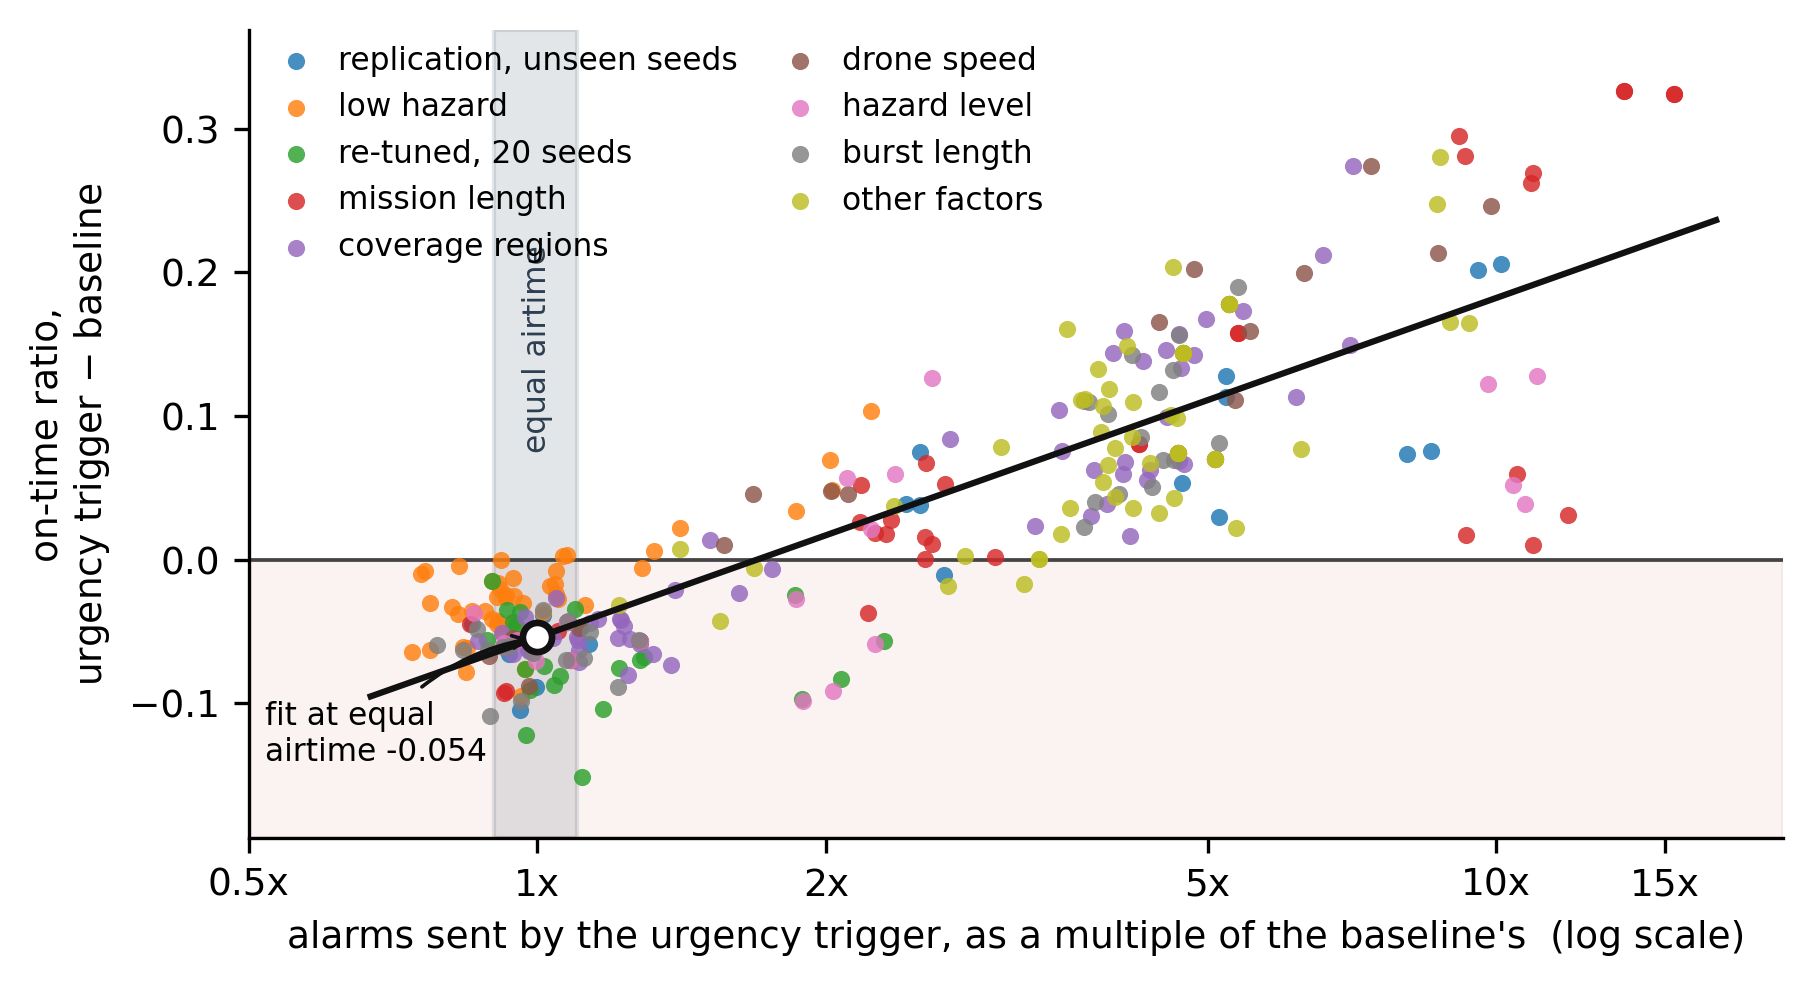
\includegraphics[width=\textwidth]{figs/fig_outspend.png}
\caption{Every paired comparison. The horizontal axis is the out-spend ratio: alarms sent
by the urgency trigger as a multiple of the baseline's. Where the two send the same
(shaded band) the baseline performs better; the apparent advantage grows with the ratio.
Colours mark the experimental factor varied (e.g.\ mission length, coverage regions); the open
circle is the fitted value at equal airtime.}\label{fig:outspend}
\end{figure*}

The ratio is not merely a proxy for the budget. At a fixed budget the relationship
remains: $r = +0.693$ at budget 11 (124 cases), $+0.779$ at 22 (20 cases) and $+0.700$ at
45 (168 cases), all $p < 10^{-4}$. At budget 5 it vanishes ($r = -0.163$, $p = 0.55$), as
expected, because every method can reach 5 alarms and the ratio barely varies.

\paragraph{A controlled test.} Lowering the hazard level puts more of the field above it,
giving the baseline more crossings on which to fire. Table~\ref{tab:ladder} fixes the budget at
45 and changes only the hazard level. The urgency trigger hits its target throughout
(44.80, 44.89, 44.91, 45.06 alarms). What changes is whether the baseline can spend its
budget, and as it loses that ability the margin turns from negative to positive.
Different hazard levels define different events (546, 634, 666 and 572 per mission, against
362 at 0.35), so on-time ratios are not comparable across rows, but the margin is, since
both methods face the same events within a row.

\begin{table}[t]
\caption{Same budget (45), four hazard levels. Ranges cover the four scenario and
coverage cases at each level.}\label{tab:ladder}
\centering
\footnotesize
\setlength{\tabcolsep}{3pt}
\begin{tabular}{@{}rrrr@{}}
\toprule
\textbf{Hazard} & \textbf{Baseline sent} & \textbf{Out-spend} & \textbf{Margin} \\
\midrule
0.10 & 36.9--49.4 & 0.92--1.07$\times$ & $-0.051$ to $+0.003$ \\
0.15 & 37.6--50.7 & 0.88--1.05$\times$ & $-0.045$ to $-0.020$ \\
0.20 & 29.8--40.9 & 1.12--1.41$\times$ & $-0.032$ to $+0.022$ \\
0.25 & 18.4--24.9 & 1.86--2.23$\times$ & $+0.034$ to $+0.104$ \\
\bottomrule
\end{tabular}
\end{table}

\subsection{At equal airtime the baseline performs better}\label{sec:equal}

In the 79 cases where both triggers sent about the same number of alarms (out-spend
0.9--1.1$\times$), the urgency trigger is worse on both measures:
\begin{itemize}
\item on-time ratio $-0.0516$, 95\% CI $[-0.0572, -0.0459]$, baseline better in
\textbf{77 of 79}, $p = 1.4\times10^{-14}$;
\item mean latency $+7.2$ ticks (later), $p < 10^{-6}$.
\end{itemize}
Figure~\ref{fig:forest} shows every case. The result holds in each of the eight
experiments that contribute matched cases, including the replication on unseen seeds and
the re-tuning with 20 seeds. Because lower hazard levels let the baseline reach 45 alarms
on target (44.98 and 45.40 at hazard 0.10 and 0.15), the matched cases span budgets 5, 11,
22 and 45, rather than only the rate at which the baseline saturates.

\begin{figure*}[t]
\centering
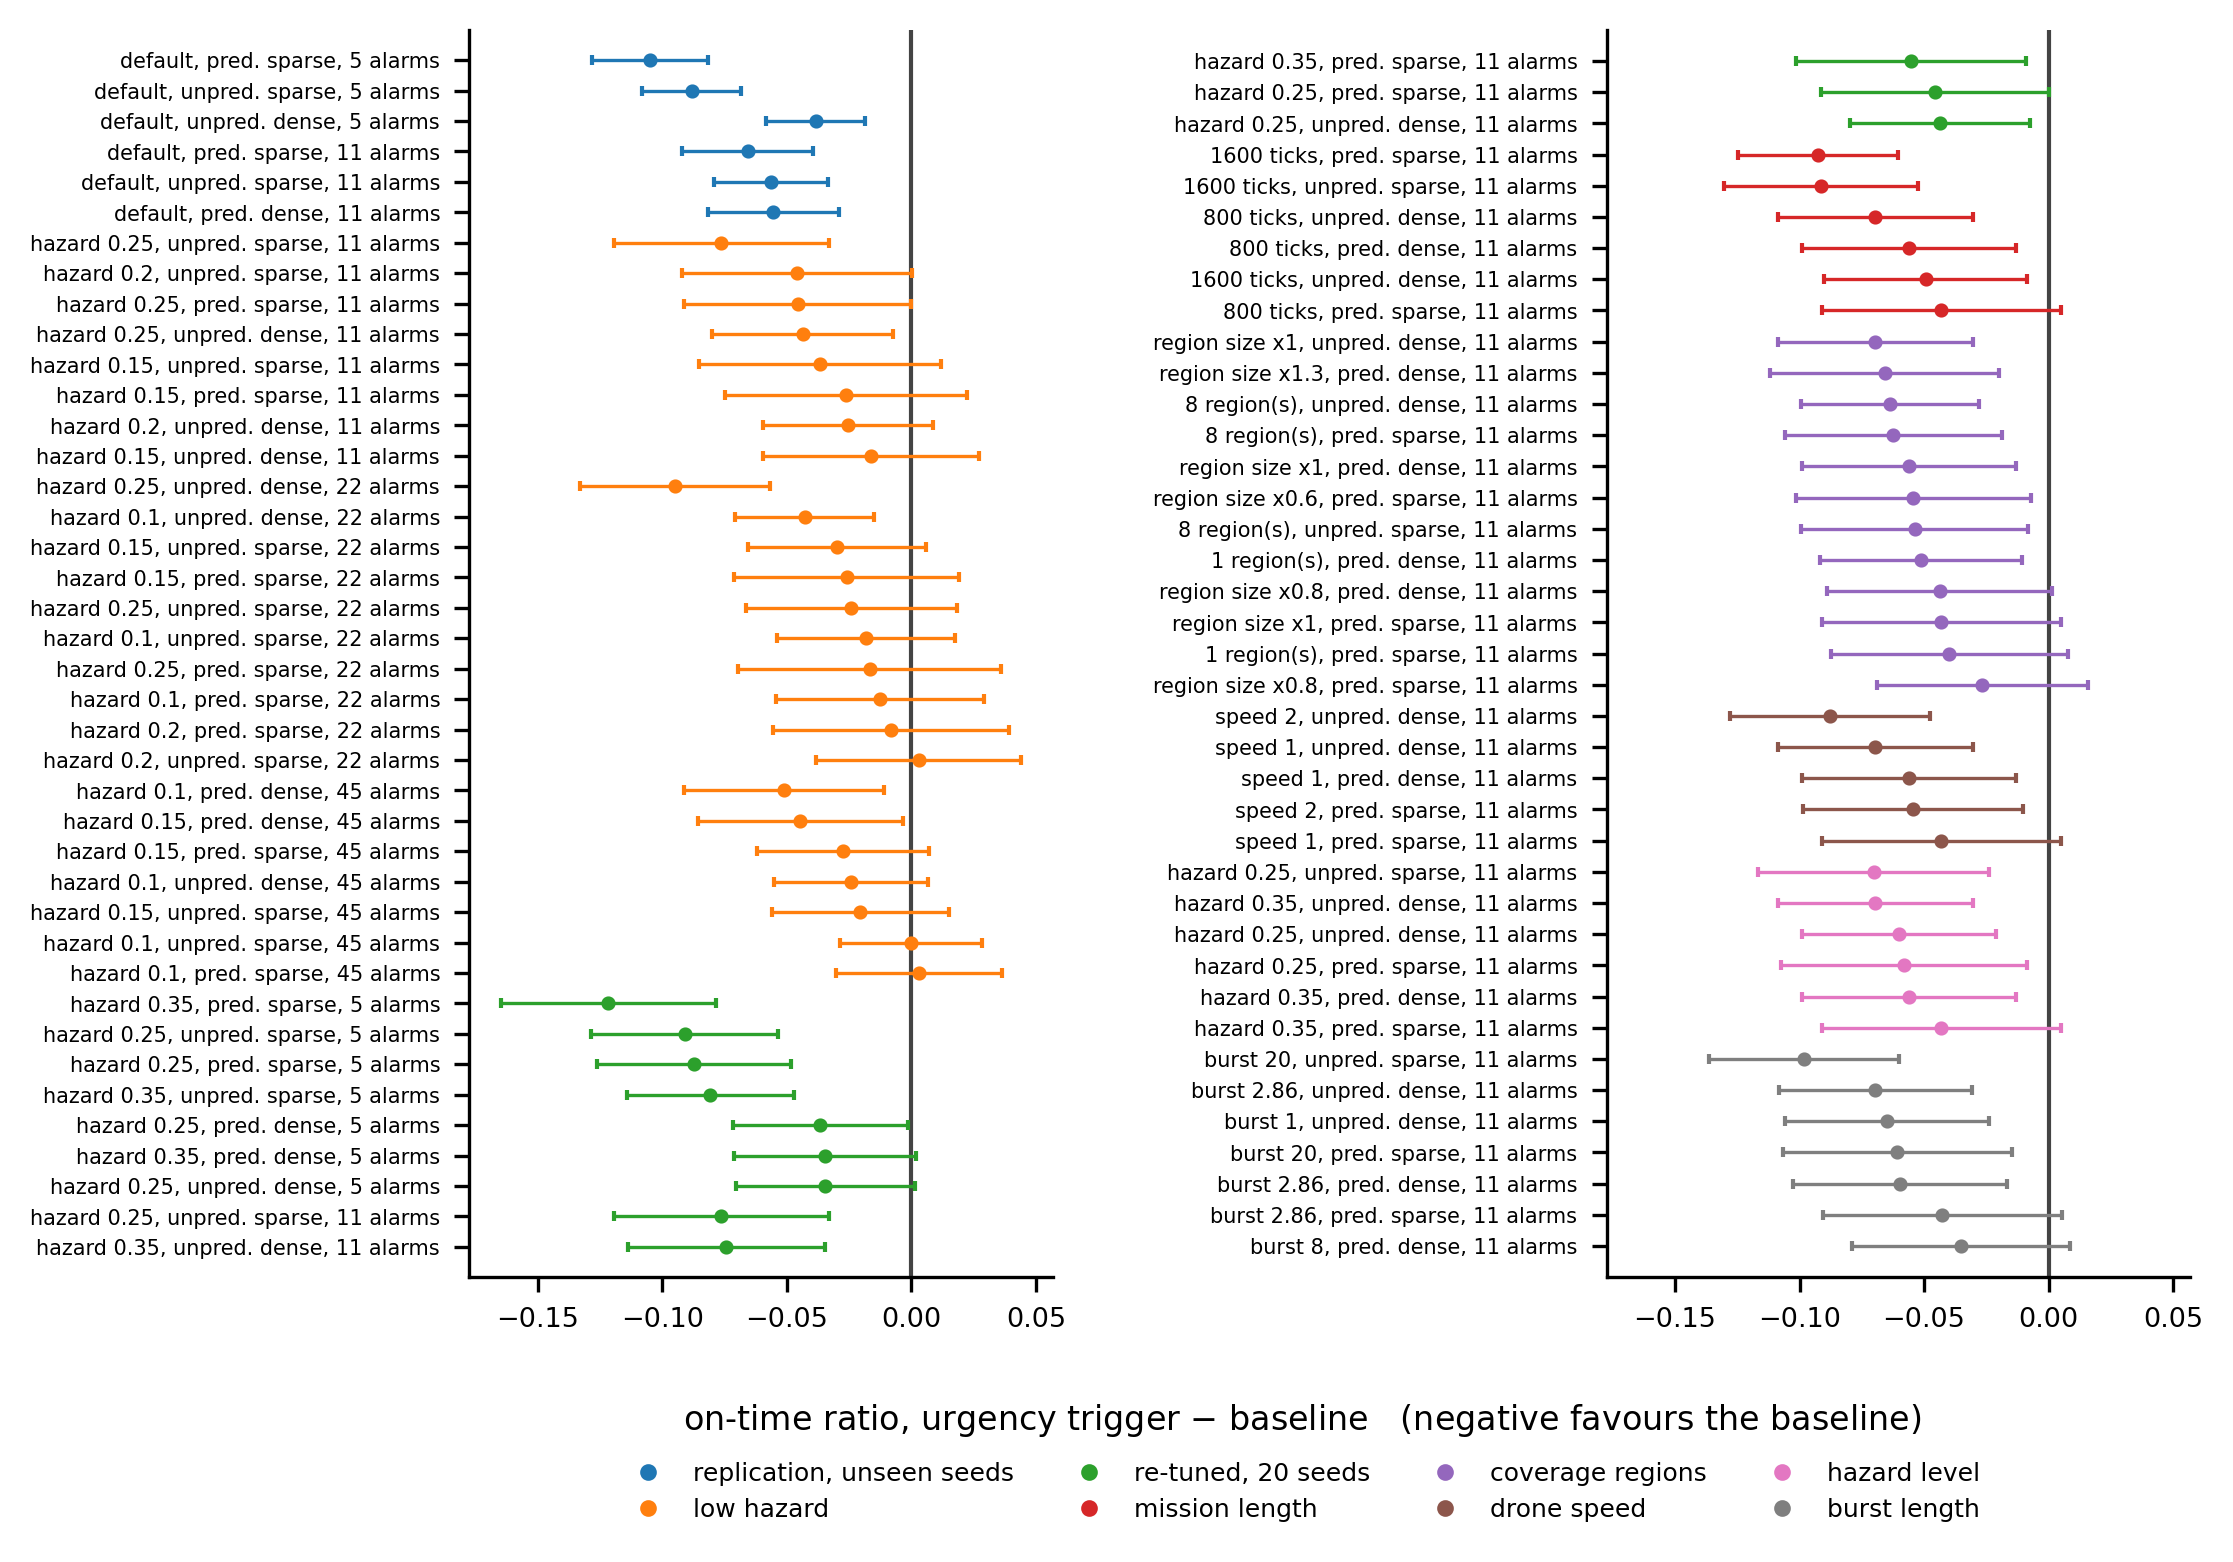
\includegraphics[width=\textwidth]{figs/fig_matched_forest.png}
\caption{The 79 cases where both triggers spent about the same airtime, with 95\%
confidence intervals. Each row gives the setting varied in that experiment (hazard level,
mission length in ticks, number or size of coverage regions, agent speed, mean burst length,
or ``default''), the field scenario (pred.\ = predictable, unpred.\ = unpredictable), the
coverage scenario and the requested budget. Colours mark the experiment. Two intervals cross
zero; the other 77 favour the baseline.}\label{fig:forest}
\end{figure*}

\subsection{The deficit narrows as the budget grows}\label{sec:narrowing}

The deficit falls about threefold as the budget rises (Table~\ref{tab:bybudget}). This is
consistent with Section~\ref{sec:discussion}: with few alarms, each is best spent on the most
clearly hazardous reading, which is what a threshold selects, so a trigger that also
responds to model error wastes a larger share of a small budget.

\begin{table}[t]
\caption{Matched cases by requested budget.}\label{tab:bybudget}
\centering
\footnotesize
\begin{tabular}{@{}rrrr@{}}
\toprule
\textbf{Budget} & \textbf{Cases} & \textbf{Mean margin} & \textbf{Baseline better} \\
\midrule
5  & 10 & $-0.0718$ & 10/10 \\
11 & 52 & $-0.0562$ & 52/52 \\
22 & 10 & $-0.0270$ & 9/10 \\
45 & 7  & $-0.0235$ & 6/7 \\
\bottomrule
\end{tabular}
\end{table}

Only two of the 79 intervals cross zero ($+0.003 \pm 0.033$ at hazard 0.10, budget 45;
$+0.003 \pm 0.041$ at hazard 0.20, budget 22), and the mean stays negative at every
budget, so this is not parity. The decoupled threshold (Section~\ref{sec:capacity})
extends the test to higher budgets at hazard 0.35: $-0.070$ at 11 alarms, $+0.011$ at 90.
At that budget the deficit closes to a tie.

\subsection{Capacity, and what removes it}\label{sec:capacity}

A capped baseline is also an operational limitation: additional bandwidth cannot be
used. The urgency trigger can use it. In the predictable, dense case its on-time ratio rises from
0.615 at budget 90 (87.5 alarms) to 0.702 at 120 (124.9) and 0.747 at 150 (157.9), and
latency falls by 36\% (71.6 to 46.1 ticks). Asking for 180 gives exactly the results of
150, so the urgency trigger has its own ceiling near 150 alarms; the gate alone would allow
about 266, and we did not isolate the rest. Energy rises 8.2\% from budget 90 to 150, but
flight dominates energy in this simulator, so that figure has limited operational meaning. Under sparse coverage, missions that deliver nothing rise from 2 to 9 of 100
with budget, so we rely on the dense case here.

The capped baseline reaches only 0.402 in this case, but that comparison is at very
unequal airtime (158 alarms against 8.5), and the cap exists only because $\max(0, o-h)$
cannot fire below $h$. We therefore tested a \emph{decoupled threshold},
\texttt{threshold\_dec}: it fires when $o > \theta$, with $\theta$ tuned freely and allowed
below $h$. Everything else is unchanged, and at $\theta = h$ it reproduces the original
baseline exactly. It ran at hazard 0.35 with 100 seeds in each of the four cases, with
predictions written before the run (Table~\ref{tab:decoupled}).

\begin{table}[t]
\caption{Urgency trigger against the decoupled threshold (B2d), hazard 0.35, 400 paired
missions per row. Ratio is the out-spend ratio; margin is urgency trigger minus B2d
on-time ratio; the CI is the normal approximation (mean $\pm 1.96$ SE). Holm-adjusted
Wilcoxon $p$: $6.2\times10^{-9}$, $0.49$ and $0.15$.}\label{tab:decoupled}
\centering
\footnotesize
\setlength{\tabcolsep}{3pt}
\begin{tabular}{@{}rrrrr@{}}
\toprule
\textbf{Budget} & \textbf{B2d sent} & \textbf{Ratio} & \textbf{Margin} & \textbf{95\% CI} \\
\midrule
11  & 11.4  & 0.96$\times$ & $-0.070$ & $[-0.092,-0.049]$ \\
90  & 91.9  & 0.96$\times$ & $+0.011$ & $[-0.012,+0.034]$ \\
150 & 139.4 & 1.09$\times$ & $+0.023$ & $[+0.001,+0.045]$ \\
\bottomrule
\end{tabular}
\end{table}

The ceiling disappears: asked for 90 alarms, the decoupled threshold sends 91.9, where the
original sends 10.4. \textbf{At 90 alarms the two triggers tie.} At 150 it reaches only
139.4, a second, smaller ceiling imposed by the gate. There the urgency trigger leads by
$+0.023$, but the lead is not significant: the normal-approximation interval only just
excludes zero, while the rank-based Wilcoxon test gives $p=0.075$, or $p=0.15$ after Holm
correction across the three budgets. The budgets are also only marginally matched, and the
lead depends on the scenario: $+0.060$ and $+0.066$ in the unpredictable cases, $-0.025$
and $-0.010$ (not significant) in the predictable ones. In the predictable, dense case above,
the decoupled threshold scores 0.771 against the urgency trigger's 0.747.

Against the capped baseline the urgency trigger gains $+0.142$ at 90 alarms and $+0.284$
at 150; against the decoupled threshold, $+0.011$ and $+0.023$. About 92\% of the
capacity advantage was the ceiling. Capacity is therefore not claimed as a general
advantage; at most there is a small edge at very high budgets in unpredictable fields.

\subsection{Sensitivity to the type of field change}\label{sec:attribution}

The unpredictable scenario combines a wind shift and a second source. Varying each
separately (8{,}000 runs, budget 45) suggests they act in opposite directions. Relative to a
steady field, an $80.2^\circ$ wind shift lowers the urgency trigger's margin from $+0.143$ to
$+0.065$ (sparse) and from $+0.106$ to $+0.026$ (dense), whereas a full-strength second
source raises it to $+0.161$ and $+0.168$. These margins are measured against the capped
baseline, and Section~\ref{sec:capacity} shows that most of such margins reflects the
ceiling, so only the ordering across shocks is informative; it is fair within each arm
because the out-spend ratio is roughly constant along it. The decoupled test provides
better evidence at matched airtime: at 150 alarms the urgency trigger leads by $+0.060$ and
$+0.066$ in the unpredictable fields and trails slightly in the predictable ones, an
indication that the surprise term helps when the field changes in ways a fitted model does
not anticipate.

\subsection{Robustness}

Nine factors were varied individually: mission length (200--1600 ticks), area size,
number (1--8) and size of coverage regions, hazard level (0.25--0.50), burst length
(1--20), agent speed (1--3), sensor noise, GP window and both gate settings. None changes
the equal-airtime result. With a single small coverage region, 26 of 27 matched cases
still favour the baseline, and an eightfold increase in burst length leaves the matched
margin unchanged, so the two-tier upload rule does not confer the predicted burst
tolerance.

%=====================================================================
\section{Comparison with Base Papers and State of the Art}\label{sec:basecmp}

No published result is directly comparable. Each reviewed work uses its own
simulator, field, channel and metric; AoI is not on-time delivery against a physical
deadline; most assume a known coverage map or several UAVs; and no public dataset
records true hazard crossings with times. We therefore \textbf{re-implement the closest
decision rules in our own simulator} as B1--B5 (Table~\ref{tab:methods}) and compare them
on identical fields, channels, seeds and budgets. All numbers in this paper come from our
implementation. Table~\ref{tab:related} lists the base papers; each optimises a stand-in
for timely hazard delivery (age, map uncertainty or throughput), and most assume away the
coverage discovery our agent must perform.

\begin{table*}[t]
\caption{Base papers. No published number is imported, because none is in units
comparable with on-time delivery; all comparisons are by re-implementation.}
\label{tab:related}
\centering
\scriptsize
\begin{tabular}{@{}P{2.6cm}P{1.0cm}P{2.0cm}P{3.0cm}P{5.6cm}@{}}
\toprule
\textbf{Work} & \textbf{Year} & \textbf{Optimises} & \textbf{Setting} &
\textbf{How we differ} \\
\midrule
AoI-optimal planning~\cite{xieAoIoptimalPathPlanning2025,
AoIOptimalMultiAAVEnabledISAC, fidler2DAoIAgeofInformationDistributed2026} & 2025--26 &
Age of Information & own simulators; known map, several agents &
AoI ignores content. Our AoI-style B3 has the worst on-time ratio measured (0.082). \\
Informative path planning~\cite{maAdaptiveInformativePath2025,
blanchardInformativePathPlanning2022} & 2022--25 & Map uncertainty & own simulators;
single agent & Optimises the map; here map accuracy trades against timeliness
(Spearman $+0.96$, Sec.~\ref{sec:ablation}). \\
Comm.-aware UAV planning~\cite{mardaniCommunicationAwareUAVPath2019,
chuTrajectoryOptimizationResource2026, hayatMultiobjectiveDronePath2020} & 2019--26 &
Throughput, outage & own simulators; \textbf{known} map &
Our agent discovers coverage in flight, recovering 3.92 of 4 regions. \\
Event-based sampling~\cite{miskowiczSendOnDelta2006,
hakandurakEfficientEventBasedSampling2026} & 2006, 2026 & Transmission count & own
simulators; static sensors &
Our B2. We show it has an alarm ceiling (8.50 per mission) that a free firing level
removes. \\
Fast GP estimation~\cite{munozGaussianProcessesFast2023} & 2023 & GP speed &
own simulator; single agent & Adopted, not compared; keeps GP cost near 20\% of runtime. \\
\bottomrule
\end{tabular}
\end{table*}

\paragraph{Improvement analysis.} Against the threshold baseline (B2) the result consists
of two numbers with opposite signs. \emph{Reach:} where B2 is capped, the urgency trigger reaches
0.747 against B2's 0.402 ($+0.345$), but at very unequal airtime (158 against 8.5 alarms),
and against the decoupled B2d the difference is only $+0.011$ at 90 alarms (a tie) and
$+0.023$ at 150 (Table~\ref{tab:decoupled}). \emph{Choosing what to send:} at equal
airtime the urgency trigger is \emph{worse} by 0.0516 in on-time ratio (about 12\% relative)
and 7.2 ticks slower, at budgets from 5 to 45. The surprise term fires on model error,
which only loosely matches hazard crossings, so with a small budget some alarms go to
readings that are surprising but harmless. These two numbers come from different operating
points, and quoting either alone misrepresents the result. Any margin reported at 22 or
more alarms per mission should come with both methods' achieved alarm rates; without them
readers cannot tell whether the budget was matched.

%=====================================================================
\section{Ablation Study}\label{sec:ablation}

Each ablation removes or replaces one component, at a matched budget of about 11 alarms per
mission, over 240 paired runs per method (Table~\ref{tab:ablation}).

\begin{table}[t]
\caption{Ablations. A negative difference means the urgency trigger is worse than that
variant.}\label{tab:ablation}
\centering
\footnotesize
\setlength{\tabcolsep}{3pt}
\begin{tabular}{@{}lrr@{}}
\toprule
\textbf{Variant} & \textbf{On-time diff.} & \textbf{$p$} \\
\midrule
\texttt{threshold} & $-0.089$ & $8.9\times10^{-9}$ \\
\texttt{raw\_abl} & $-0.066$ & $1.2\times10^{-6}$ \\
\texttt{fixed\_dl} & $-0.033$ & $3.7\times10^{-3}$ \\
\texttt{surprise\_abl} & $-0.005$ & $0.71$ \\
\texttt{always\_tx} & $+0.146$ & $5.0\times10^{-25}$ \\
\texttt{time\_urg} & $+0.196$ & $1.0\times10^{-36}$ \\
\bottomrule
\end{tabular}
\end{table}

\paragraph{Routing is the method's main benefit.} Transmitting in place instead of
selecting an upload point costs 0.146 on-time ratio, and replacing the content trigger with
a timer costs 0.196. These are the largest effects measured.

\paragraph{The consequence term has no measurable effect at a small budget.} Removing it
changes the on-time ratio by $-0.005$ ($p = 0.71$).

\paragraph{Uncertainty scaling and urgency deadlines are trade-offs.} Dividing surprise by
$\sigma$ lowers on-time delivery (0.278 against 0.345) but improves map accuracy (0.224
against 0.257), and urgency deadlines cost 0.033 against fixed ones.

\paragraph{Delivery and map accuracy trade off.} Across the seven methods, on-time ratio and
map RMSE rise together (Spearman $+0.96$; Pearson $r = +0.89$, $p = 0.007$). Since lower
RMSE is better, better delivery comes with a worse map. \texttt{time\_urg} has the worst
on-time ratio (0.082) and the best map RMSE (0.194), because map RMSE largely measures how
evenly the uploads are spread. We therefore treat map RMSE as a diagnostic, never as a
second headline.

\paragraph{The gate mainly throttles the baseline.} Raising $k$ from 1 to 5 raises the
out-spend ratio from $1.4\times$ to $9.0\times$, and the apparent margin from $+0.008$ to
$+0.247$. At $k=1$, where airtime is closest to equal, the margin is within noise.

%=====================================================================
\section{Discussion}\label{sec:discussion}

\paragraph{Why the method behaves as it does.} The urgency trigger fires on \emph{model
error}. When the budget is small compared with the number of hazard events (about 11
alarms against 370 observable events per mission), the best policy is to spend every alarm
on the reading most clearly above the hazard line. A threshold does exactly that. A
surprise term does not, because model error and hazard crossings are only loosely
related, so some alarms go to surprising but harmless readings. The measured detection
rate (8.9\% against 11.8\%) and false-alarm rate (0.255 against 0.201) agree.

The capacity result required an unanticipated correction. The capped baseline's alarm
count was limited by how much of the field is above the hazard level, but that limit came
from the setup, not from threshold triggering: a threshold with a free firing level can be
tuned to almost any rate. Once both triggers can spend a large budget, the reading itself
is nearly as informative as the model's surprise, and the two tie.

\paragraph{Was the research gap addressed?} Partly, and not in the intended direction. The
gap was that content-aware triggering and connectivity-aware routing are usually studied
separately. The routing half is supported: coverage discovery works (3.92 of 4 regions
found), flying to a found region is chosen 37--44\% of the time, and removing upload-point
choice costs 0.146 on-time ratio. The triggering half is \emph{not} supported at a matched
budget, and the fallback claim, that the urgency trigger at least offers more capacity,
does not hold against a decoupled threshold beyond a small, scenario-dependent edge at
150 alarms.

\paragraph{Threats to validity.} Everything is simulated, so absolute values depend on the
field, channel and energy models; only the relative and structural findings should be
carried over. Energy is dominated by flight, which makes alarms unusually cheap, and a
comparison at matched \emph{energy} rather than matched alarms has not been done; it is
the most important gap left. All missions use a single agent in one simulator. The
shrinking of the deficit with budget rests on only 17 matched cases at budgets 22 and 45,
so its slope is less certain than its sign, and the decoupled threshold was tested in one
configuration only. Three candidate explanations for the deficit were rejected by the data, so no
mechanism beyond the one above is claimed.

%=====================================================================
\section{Conclusion and Future Work}\label{sec:conclusion}

A hazard-threshold trigger for mobile sensing has a hard alarm ceiling, 8.50 alarms per
mission even at a trigger of zero, because its firing level is the hazard level itself.
Above that ceiling a matched alarm budget is matched in name only: across 332
comparisons the urgency trigger's margin follows how many more messages it sends
($r = +0.861$). Where airtime is genuinely equal, the threshold performs better in 77 of 79 cases
and delivers 7.2 ticks sooner, from 5 to 45 alarms per mission and on unseen seeds. The
urgency trigger's large lead over the capped baseline (0.747 against 0.402) does not
survive a fairer baseline: a threshold free to fire below the hazard level sends 92 alarms
per mission and ties it at that budget. The pre-registered success rule was not met.
The method's clear contribution is its routing: selecting the upload point is worth
0.146 on-time ratio.

Future work includes a matched-energy comparison, which is the question an operator would ask;
repeating the decoupled-threshold test across hazard levels, agent speeds and gate sizes
to see whether the tie at high budgets is general; and the simple practice of reporting
achieved alarm rates next to every matched-budget result, so that readers can distinguish capacity
from better selection.

\backmatter

\bmhead{Data and code availability}
The simulator, the frozen protocols, the raw run archives and the analysis scripts that
regenerate every table and figure in this paper are available in the project repository at
\url{https://github.com/fatima-1206/urgency-sim}. Every result row carries a git commit hash, a configuration
hash and library versions, and each frozen protocol is identified by the commit at which
it was fixed.

\bmhead{Declarations}
\textbf{Conflict of interest.} The authors declare no competing interests.
\textbf{Funding.} No funding was received for this work.
\textbf{AI-tool usage.} An AI coding assistant (Anthropic Claude) was used for simulator
implementation, experiment orchestration, analysis scripting and drafting assistance.
All experimental designs, pre-registered protocols, success rules and scientific
conclusions are the authors' own, and all reported numbers were generated by the
committed code and are reproducible from the archived runs.

\bibliography{references}

\end{document}
